\section{Communicating Results \& Project Preparation}

\begin{frame}{Visualisation Matters}
  \begin{center}
    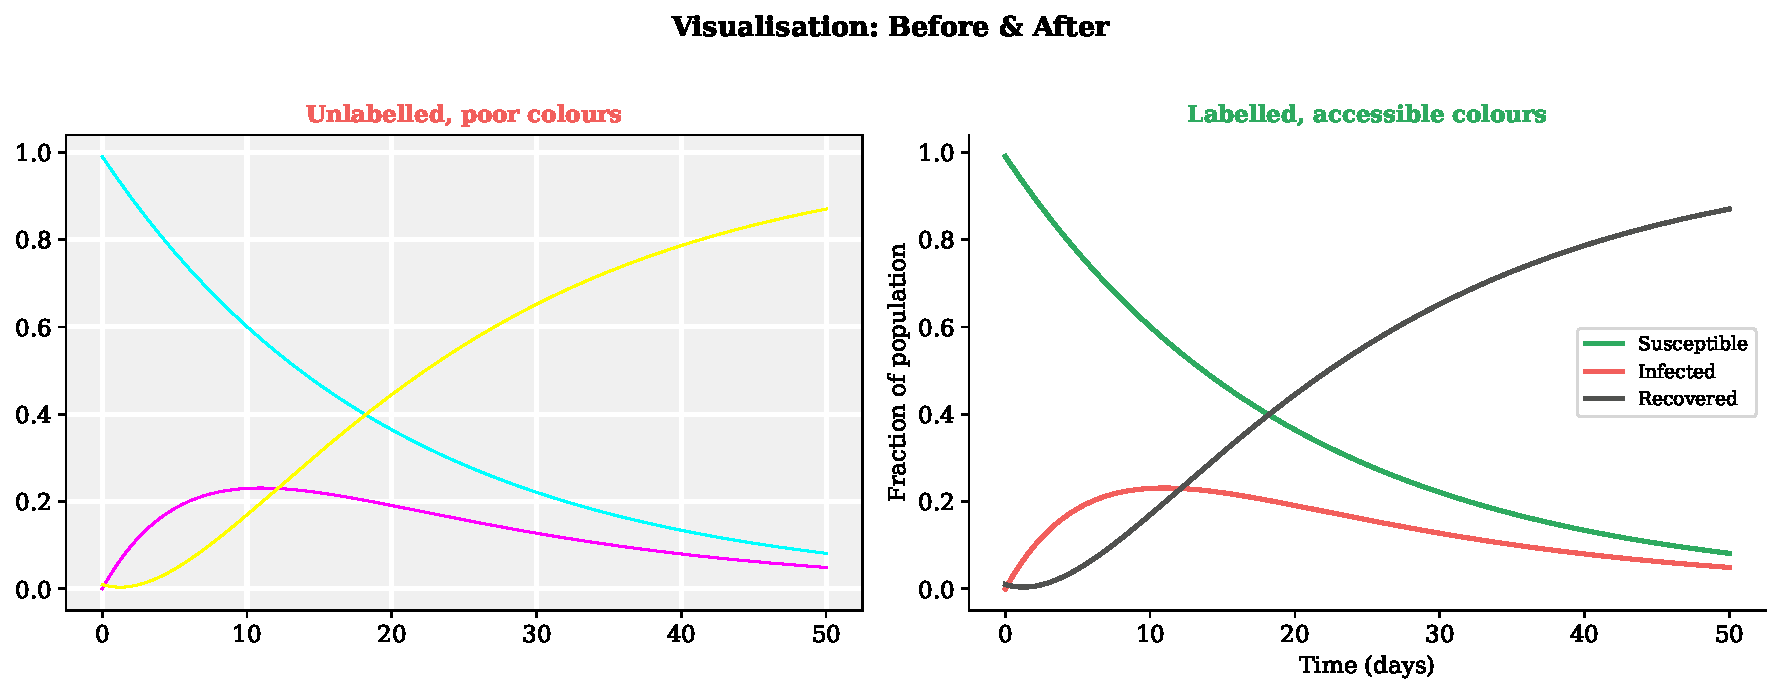
\includegraphics[width=0.95\textwidth]{images/good_vs_bad_viz.pdf}
  \end{center}
  \begin{itemize}
    \item Your plots are the \textbf{first thing} reviewers and audiences see.
    \item Bad visualisation can hide correct results; good visualisation can illuminate them.
  \end{itemize}
\end{frame}

\begin{frame}{Visualisation Checklist}
  Every figure in your report should have:
  \begin{enumerate}
    \item \textbf{Axis labels} with units (e.g.\ ``Time (days)'', ``Population $N$'').
    \item \textbf{Legend} or direct labels --- the reader should never guess which line is which.
    \item \textbf{Accessible colours} --- avoid red/green only combinations (colour-blind readers).
    \item \textbf{Caption} that describes what the reader should see.
    \item \textbf{Consistent style} across all figures in the report.
  \end{enumerate}
  \medskip
  Tools: \texttt{matplotlib} defaults are decent; use \texttt{plt.rcParams} to set a global style once.
\end{frame}

\begin{frame}{Structuring Your Project Report}
  Recommended structure (4--6 pages + code):
  \medskip
  \begin{description}
    \item[1. Introduction] What system are you modelling? Why is it interesting?
    \item[2. Model Description] Equations, rules, parameters, assumptions. Include a diagram.
    \item[3. Implementation] Key code design decisions. Not a code dump --- highlight the important parts.
    \item[4. Results] Figures with captions. What do the simulations show?
    \item[5. Analysis] Sensitivity analysis, parameter sweeps, comparison to data or simpler models.
    \item[6. Discussion] What did you learn? What are the limitations? What would you do next?
  \end{description}
\end{frame}

\begin{frame}{Writing About Models: Do's and Don'ts}
  \textbf{Do:}
  \begin{itemize}
    \item State all assumptions explicitly.
    \item Provide parameter values and their sources.
    \item Discuss what the model \emph{cannot} capture.
    \item Compare against a baseline (simpler model, analytical solution, or data).
  \end{itemize}
  \medskip
  \textbf{Don't:}
  \begin{itemize}
    \item Claim the model ``proves'' something --- models \emph{suggest} or \emph{are consistent with}.
    \item Present only the best-looking run out of many.
    \item Ignore parameters you did not vary.
    \item Skip units or dimensional analysis.
  \end{itemize}
\end{frame}


\begin{frame}{Recap: The Modelling Workflow}
  \begin{enumerate}
    \item \textbf{Define the question.} What behaviour do you want to understand or predict?
    \item \textbf{Choose the paradigm.} ODE, CA, ABM --- use the decision flowchart.
    \item \textbf{Implement.} Start simple. Verify against known solutions.
    \item \textbf{Explore.} Sweep parameters. Run ensembles. Compare to data.
    \item \textbf{Validate.} Does it reproduce the qualitative / quantitative behaviour?
    \item \textbf{Communicate.} Figures, report, presentation.
  \end{enumerate}
  \medskip
  \begin{center}
    \textbf{Good luck with your projects!}
  \end{center}
\end{frame}
